% =====================================================================
% 4  Power and publication bias        Folien 11-13 | 4:45 min | bis 16:15
% Inhalt: Bericht Kap. 6-7. Pflicht laut instruction.pdf: Funnel Plot und
% eine Aussage zur visuellen Evidenz fuer Publication bias.
% Backup A3 (Power-Robustheit) und A4 (alle Stichproben) verlinkt.
% Von Hand getippte Zahlen (kein Makro) sind unten markiert.
% =====================================================================
\section{Power and publication bias}

% ---------------------------------------------------------------------
\begin{frame}[label=power]{Statistical power}
  \timing{1:30}{13:00}
  \begin{columns}[T]
    \begin{column}{0.55\textwidth}
      \centering
      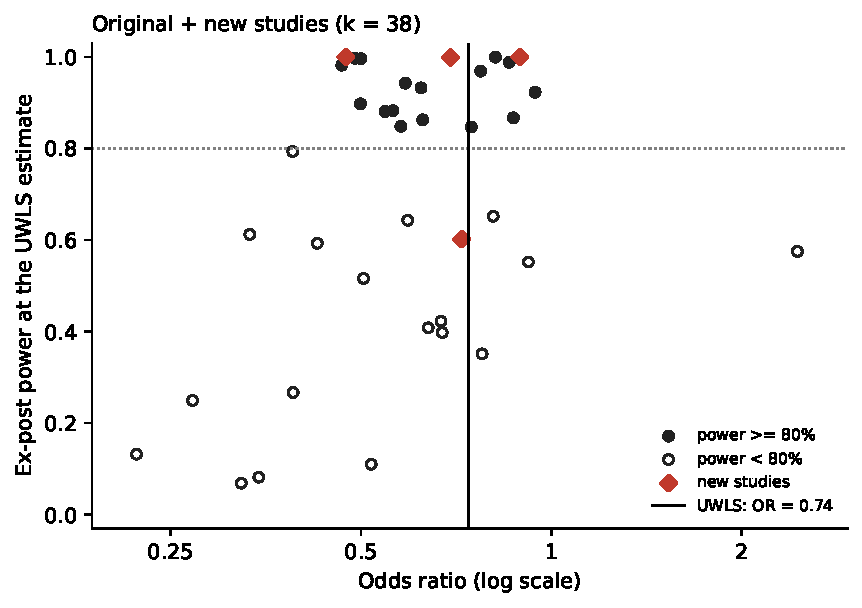
\includegraphics[width=\linewidth]{power_combined}
    \end{column}
    \begin{column}{0.43\textwidth}
      \[ q_i = \Phi\!\left( \frac{|\hat\mu_{UWLS}|}{SE_i} - 1.96 \right) \]
      \begin{itemize}
        \item \textbf{Median power:} \maMedPower{} (original),
          \maMedPowerComb{} (with new studies)
        \item \textbf{Adequately powered} ($q_i \geq 0.8$): \maNadequate{}
          of \maK{} / \maNadequateComb{} of \maKcomb
        \item Leading economics journals: median power only 7\,\%
          \citep{askarov2024}% 7 % von Hand (Bericht Kap. 6)
      \end{itemize}
    \end{column}
  \end{columns}
  \keymsg{Correspondence tests are well powered; the drop after the update
    reflects a smaller benchmark effect, not weaker studies.}
  \buttons{\gotobackup{app-power}{Robustness}}
\end{frame}
% Sprechnotizen (Folie 11):
% - Grafik: jeder Punkt = eine Studie; x = OR, y = Power; gestrichelt = 80 %.
% - Formel: wahrer Effekt = UWLS-Schaetzer. Adequately powered heisst
%   SE_i <= |mu| / 2.8 (1.96 + 0.84 = 2.8).
% - Warum sinkt die Power nach dem Update? Kline zieht UWLS gegen 1; ein
%   kleinerer angenommener Effekt senkt die Power ALLER Studien. Ohne Kline:
%   Median 0.99 (Backup A3).
% - Einschraenkung: eher Obergrenze (nur publizierte Studien; der
%   Benchmark-Effekt kann selbst durch Publication bias aufgeblaeht sein).

% ---------------------------------------------------------------------
\begin{frame}{Publication bias: visual evidence}
  \timing{1:30}{14:30}
  \begin{columns}[T]
    \begin{column}{0.58\textwidth}
      \centering
      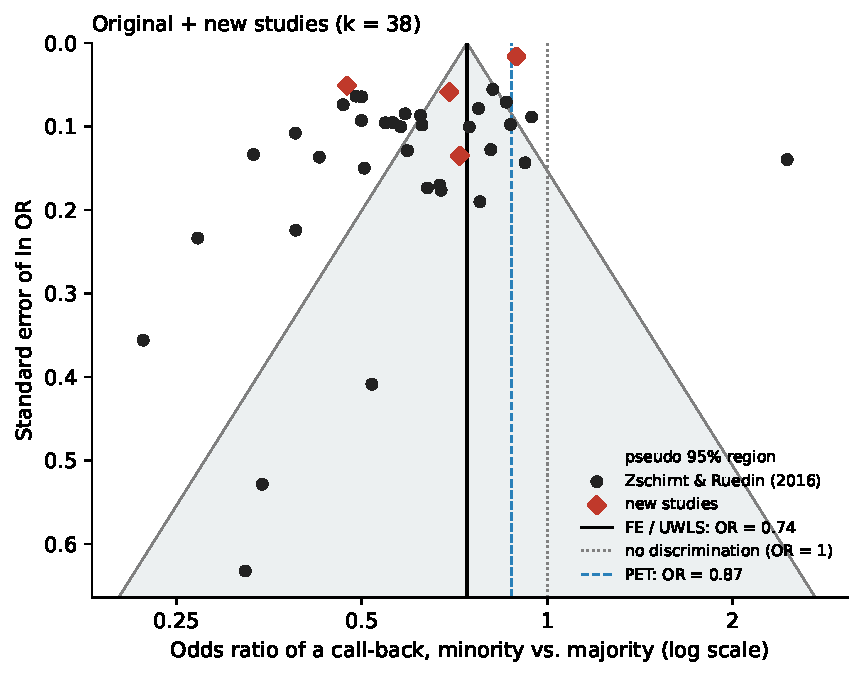
\includegraphics[width=0.92\linewidth]{funnel_combined}
    \end{column}
    \begin{column}{0.40\textwidth}
      \begin{itemize}
        \item \textbf{Asymmetric:} 15 of 19 less precise studies lie left of
          the UWLS estimate, i.e.\ report stronger discrimination% 15 of 19 von Hand (Bericht Kap. 7)
        \item \textbf{New studies} (red): three are among the four most
          precise studies, yet range from \maORnewMin{} to \maORnewMax
        \item \textbf{Caveat:} with $\ln OR$, effect and SE are
          mechanically correlated
      \end{itemize}
    \end{column}
  \end{columns}
  \keymsg{Asymmetric funnel: consistent with publication bias, but also with
    heterogeneity.}
\end{frame}
% Sprechnotizen (Folie 12):
% - Lesen: oben praezise, unten unpraezise Studien. Ohne Bias symmetrisch
%   um die durchgezogene Linie (FE/UWLS 0.74). Blau gestrichelt = PET (0.87),
%   gepunktet = OR 1 (keine Diskriminierung).
% - Viele praezise Studien liegen ausserhalb des grauen Pseudo-95%-Bereichs
%   -> grosse Heterogenitaet.
% - Neue Studien: Kline (Rang 1), Adamovic (2) und Koopmans (4) sind sehr
%   praezise; Zschirnt & Fibbi liegt in der unpraeziseren Haelfte (Rang 24).
% - Caveat: der SE haengt von den Callback-Zahlen ab, diese von der
%   Callback-Rate -> Asymmetrie ist kein Beweis fuer Bias.

% ---------------------------------------------------------------------
\begin{frame}[label=bias]{Correcting for publication bias}
  \timing{1:45}{16:15}
  \vspace{-0.5em}
  \[
    y_i = \beta_0 + \beta_1 SE_i + \varepsilon_i, \quad w_i = 1/SE_i^2
    \qquad \text{FAT: } H_0\!: \beta_1 = 0, \quad \text{PET: } \hat\beta_0
  \]
  \centering\small
  \begin{tabular}{lcc}
    \toprule
    & Original ($k = \maK$) & Original + new ($k = \maKcomb$) \\
    \midrule
    RE (REML), OR      & \maORre{} \maCIre       & \maORcomb{} \maCIcomb \\
    WAAP, OR           & \maORwaap{} \maCIwaap   & \maORwaapComb{} \maCIwaapComb \\
    PET, OR            & \maORpet{} \maCIpet     & \maORpetComb{} \maCIpetComb \\
    FAT: $\hat\beta_1$ (SE) & \maFAT{} (\maFATse) & \maFATComb{} (\maFATseComb) \\
    ESS (observed $-$ expected) & \maESS        & \maESSComb \\
    \bottomrule
  \end{tabular}

  \raggedright\normalsize
  \begin{itemize}
    \item \textbf{Original:} FAT insignificant, ESS $\approx 0$
      $\Rightarrow$ little sign of bias
    \item \textbf{With new studies:} significant FAT, excess significance,
      PET moves to \maORpetComb{} -- driven by \citet{kline2022}
  \end{itemize}
  \keymsg{Evidence of bias appears only once the very precise US study is
    included; all corrected estimates stay below 1.}
  \buttons{\gotobackup{app-bias}{All samples}}
\end{frame}
% Sprechnotizen (Folie 13) -- schwierigste Folie, Zeit nehmen:
% - FAT (beta_1): Bei Diskriminierung ist ln OR < 0. Eine unpraezise Studie
%   braucht einen STAERKER negativen Effekt, um signifikant zu sein. Wird
%   nur Signifikantes publiziert -> beta_1 < 0. Kombiniert: -3.16 (SE 0.86).
% - PET (beta_0): Effekt einer hypothetischen Studie mit SE -> 0 = korrigierter Effekt.
% - WAAP: UWLS nur ueber Studien mit Power >= 80 %; aendert kaum etwas
%   (0.76 vs. 0.74), weil UWLS die schwachen Studien ohnehin kaum gewichtet.
% - ESS: 31 von 38 signifikant (0.82), erwartet laut Power nur 0.68.
% - Muendlich (von Hand gerechnet, nicht auf der Folie): ohne Kline ist die
%   Steigung -0.40 (SE 1.21), nicht signifikant, PET-OR 0.64.
